A modificação, de forma controlada, no comportamento de um sistema, garantindo uma maior eficiência é o objetivo do controle de sistemas, que é estudado desde os antigos, mas que obteve grande relevância na necessidade trazida com a revolução industrial, e hoje conta com o seu segmento específico da engenharia, com diversos trabalhos nessa área e uma infinidade de aplicações. 
 

A principal tarefa de um engenheiro é,
"o processo de concepção ou invenção de formas, partes e detalhes de
um sistema para alcançar um propósito específico"
\cite{dorf2011modern},
processo este que soma a grande capacidade de análise e a criatividade para atender as demandas da função, como é o caso de projeto em engenharia no segmento de Sistemas de Controle, cujo objetivo é obter a configuração, as especificações e a identificação de processos para atender uma necessidade real. 


Uma concepção semelhante é
"Um sistema de controle consiste em subsistemas e processos(ou plantas) construídos com o objetivo de se obter uma saída desejada com desempenho desejado para uma entrada específica fornecida"
\cite{nise2009engenharia}.


Os sistemas de controle atuam basicamente gerando respostas específicas para estímulos específicos de forma controlada e automática, trazendo vantagens nas aplicações em diversas áreas, tais como, 
na movimentação de grandes equipamentos com precisão, em locais remotos ou perigosos, na compensação de perturbações, manipulando os dados de forma conveniente.



Tanto sistemas de controle, como as mais diversas formas de transcrever o mundo físico, os sistemas de engeharia, computação, eletrônica, por exemplo, passam pelo paradigma da lógica clássica, sendo tal visão cunhada por Aristóteles na forma lógica de lidar com o mundo, que estabeleceu as regras que permearam a história até o presente momento, e seguirão válidas por um prazo ainda indeterminado, mas que, no século XX foram questionadas, procurando-se novas formas e ferramentas para tratar de questões que fogem das regras vigentes, como o tratamento de contradições e incertezas. A Lógica Paraconsistente é uma das ferramenta que se apresenta com o potencial de ir além dos limites da lógica clássica.

A Lógica Paraconsistente Anotada Evidencial $\tau$ (LPA$E\tau$) é a uma vertente da Lógica Paraconsistente que vem sendo explorada para finalidades práticas, tais como o reconhecimento de padrões em banco de dados, tomada de decisão e tratamento de incertezas em sistemas robóticos e logísticos, mas todas as áreas com uma abordagem ligada à Inteligência Artificial ou ao controle discreto do processo, ainda há escassez de trabalhos no controle contínuo de sistemas dinâmicos. 


A análise da implementação da LPA$E\tau$ no universo das lógicas não-convencionais implica em possibilitar uma nova forma de controle de sistemas, sua definição permite um embasamento para criar novas possibilidades de seu uso, e ajudar a sedimentar a nova ferramenta no meio acadêmico. 



%%%%%%%%%%%%%%%%%%%%%%%%%%%%%%%%%%%%%%%%%%%%%%%%%%%%%%%%%%%%
%\section{Hipótese e Relevância do Trabalho}
%%%%%%%%%%%%%%%%%%%%%%%%%%%%%%%%%%%%%%%%%%%%%%%%%%%%%%%%%%%%
%A Lógica Paraconsistente Anotada Evidencial $E\tau$ 
%pode ser utilizada para o controle de sistemas dinâmicos, 
%hipótese esta que confirmada pode elevar ainda mais a sua relevância e 
%elencar mais uma alternativa para aplicações técnicas e científicas. 

A lógica paraconsistente vem ganhando relevância e adeptos 
principalmente a partir do final da década de 90 do século XX, 
quando houve o Primeiro Congresso Mundial sobre 
Paraconsistência em Gent na Bélgica em 1997, 
no ano 2000 o segundo congresso realizado em São Sebastião, São Paulo e o 
terceiro em Toulouse, França em julho de 2003, 
atraindo cada vez mais pesquisadores interessados de 
diversos centros de pesquisa do mundo \cite{DecioKrause}. 

Em meados de setembro de 2016, 
aconteceu o pela primeira vez no Brasil a 
XVI Conferência Internacional de Lógica: 
\texttt{Tendências da Lógica} (\emph{Trends In Logic XVI - 
Studia Logica International Conference}) \cite{trendsinlogic}, 
realizada pelo Centro de Lógica, Epistemologia e História da Ciência (CLE) da 
Universidade Estadual de Campinas, 
que reuniu estudiosos brasileiros e de diversos países com 
trabalhos e apresentações sob o tema: 
Consistência, Contradição, Paraconsistência e Racioncínio 
(\emph{Consistency, Contradiction, Paraconsistency, and Reasoning}).

Atualmente as pesquisas estão focadas no estudo da 
aplicação da Lógica Paraconsistente, 
e ganhar espaço no universo técnico e científico, 
contribuindo com uma nova e eficiente forma de trabalho.










\section{Lógica Não-Convencional}




%O controle moderno trata de sistemas multivariáveis, 
%não lineares ou variantes no tempo 
%de forma mais apropriada do que o controle clássico, 
%reduzindo a complexidade das expressões para que 
%haja a possibilidade de um processamento satisfatório.
%Dentro do universo do controle moderno, 
%existe ainda o controle convencional que utiliza a 
%análise de sistemas de controle no espaço de estados, 
%que utiliza n-equações de primeira ordem 
%combinadas em uma equação diferencial vetor-matricial, 
%de forma a simplificar e possibilitar 
%o trabalho com uma quantidade de variáveis alta 
%sem que haja um grande impacto no processamento
%\cite{Ogata}.
O controle não convencional, 
que também é classificado como controle moderno e que
apresenta uma grande diversidade de técnicas, 
tais como o controle adaptativo, 
algorítmo adaptativo e genético, 
redes neurais, 
as lógicas Fuzzy e Paraconsistente, 
esta última sendo o alvo da abordagem do presente trabalho, 
entre outras.


A lógica, como ramo filosófico que trata das 
relações de coerência racional e discursiva, proposições e conclusões, 
tem como origem a Grécia Antiga com o seu primeiro arranjo formal em 
\emph{Tópicos} de Aristóteles por volta de 340 a.C. 
Apesar de suas bases serem conhecidas e discutidas por 
diversos pensadores anteriores, 
não havia a formalização de uma teoria bem fundada, 
apenas o tratamento de ideias como 
consistência e consequências da contraditoriedade por exemplo. 

Os princípios da lógica enunciadas por Aristóteles são 
basilares para a teoria clássica e 
moldaram o pensamento e a noção de consistência, ou não contraditoriedade, 
estreitamente conectadas ao conceito de completude e 
podem ser descritos formalmente assim:


\begin{enumerate}
\item Princípio de Identidade: 
    \begin{math}
	A \rightarrow B 
	\textrm{ ou } 
	\forall x(x=x);
    \end{math}

\item Princípio do Terceiro Excluído:
    \begin{math}
	A \vee \neg A
	\textrm{ ou }
	\forall x(Ax \vee \neg Ax);
    \end{math}

\item Princípio da Não Contradição: 
    \begin{math}
	\neg (A \wedge \neg A)
	\textrm{ ou }
	\forall x\neg(Ax \wedge \neg Ax).
    \end{math}

\end{enumerate}

O grande desenvolvimento da lógica, 
principalmente nos séculos XIX e XX, 
forneceu ferramental para caracterização e 
tratamento preciso da lógica clássica 
e também possibilitou o desenvolvimento de sistemas lógicos não clássicos, 
rearranjos, experimentações e 
questionamentos de dogmas secularmente estabelecidos.

Uma questão que já havia sido objeto de estudo por diversos pensadores desde os pré-socráticos, 
como Heráclito e sua doutrina da harmonia dos opostos, 
é a questão da contradição, 
que por vezes incomodou-os 
mas que nunca havia sofrido um tratamento formal 
como o desenvolvido por 
Newton C. A. da Costa(1929-presente data) e 
Stanislaw Jaskiwski(1906-1965), 
que propuseram e desenvolveram sistemas lógicos que fossem capazes de lidar com essas inconsistências \cite{DecioKrause}. 





%%%%%%%%%%%%%%%%%%%%%%%%%%%%%%%%%%%%%%%%%%%%%%%%%%%%%%%%%%%
\section{A Lógica Paraconsistente}
%%%%%%%%%%%%%%%%%%%%%%%%%%%%%%%%%%%%%%%%%%%%%%%%%%%%%%%%%%%





Ao restringir-se o princípio da não contradição, 
em um certo sistema lógico, 
obtém-se um resultado que pertence à lógica denominada Paraconsistente, 
desenvolvida por da Costa e Jaskiwski. 

%Para (da Costa e Marconi, 1989), ao restringir em um certo sistema lógico o princípio da não contradição, obtém-se um resultado que pertence à lógica denominada Paraconsistente.


Assim sendo, para uma dada teoria, 
se houver um símbolo de negação, 
como por exemplo "\emph{$\neg $}", 
se em qualquer fórmula fechada \emph{A} não for demonstrável \emph{$A$} e \emph{$\neg A $}, 
a teoria é consistente (não contraditória), 
senão, ela é inconsistente(contraditória).


Teoria é definida por Gomes(\citeyear{Gomes2013} p.4) como sendo:
\citacao
{
...um conjunto de fórmulas(expressões bem formuladas) de uma linguagem, 
fechadas por uma determinada relação de consequência, 
que caracteriza a lógica subjacente à teoria, 
da qual ela herda todas as suas características estruturais como, 
por exemplo, consistência(não contraditoriedade) e completude.
}

Na lógica clássica, 
uma teoria é completa, 
se e somente se, for consistente para toda a fórmula fechada \emph{A} 
onde \emph{A} e \emph{$\neg A$} é teorema da teoria 
e a teoria é trivial ou supercompleta se todas as fórmulas expressáveis forem demonstráveis, 
tanto \emph{A} quanto \emph{$ \neg A$}.


Sendo que toda a lógica paraconsistente, 
não se pode deduzir qualquer fórmula à partir de uma fórmula \emph{A} e sua negação \emph{$\neg A$}, 
mostrando assim que as noções de inconsistência (contraditoriedade) e trivialidade são de fato independentes.



%A lógica paraconsistente, segundo (Evandro Luis Gomes, 2013) 
%"Apesa do problema da existência de contradições aceitáveis já vir chamando a atenção de lógicos e filósofos pelo menos desde o tempo de Aristóteles, até o aparecimento das lógicas paraconsistentes não se dispunha de um aparato lógico para o estudo das contradiçẽos." 
%Arruda(1990, p.5-6) in Evandro Luis Gomes, 2013 p.5

%"E, como da Costa mesmo reconhecera antes, em 1958, a não trivialidade é que é decisiva ao exercício teórico-racional."
%Evandro Luis Gomes, 2013 p.439



%%%%%%%%%%%%%%%%%%%%%%%%%%%%%%%%%%%%%%%%%%%%%%%%%%%%%%%%%%%%
\subsection{Reticulado de Hasse}
%%%%%%%%%%%%%%%%%%%%%%%%%%%%%%%%%%%%%%%%%%%%%%%%%%%%%%%%%%%%

A Lógica Paraconsistente sendo apropriada para tratar dados inconsistentes foi utilizada em 1987, 
por H. Blair e V. S. Subrahmanian para representar e codificar o funcionamento de bancos de dados inconsistentes. 
\cite{Abe1992} 
Pouco depois Costa, Subrahmanian e Vago propuseram a lógica paraconsistente anotada e sua extensão a uma lógica de predicados paraconsistente anotada de primeira ordem. 

Nas Lógicas Paraconsistentes Anotadas, uma proposição $P$ utiliza um reticulado formado por pares ordenados tal que: 

\begin{center}
\begin{equation}
\tau = \{ ( \mu , \lambda ) \mid \mu ,\lambda \in [0,1] \subset \Re \}
\end{equation}
\end{center}

de acordo com graus de evidência das constantes anotacionais do reticulado 
associado à Lógica Paraconsistente Anotada Evidencial $E\tau$, 
formalmente descritas como 

\begin{center}
\begin{equation}
  \tau = \{ \top , V, F, \bot \}
\end{equation}
\end{center}

os quais descrevem os extremos do reticulado como sendo 
inconsistente,% ($\top$), 
verdadeiro, %(V), 
falso e % (F) e 
paracompleto,% ($\bot$), 
respectivamente, e são representadas conforme Figura \ref{fig:reticuladoHasse}; 




%\begin{figure}[!htb]
%\caption{Reticulado finito de Hasse}
%\center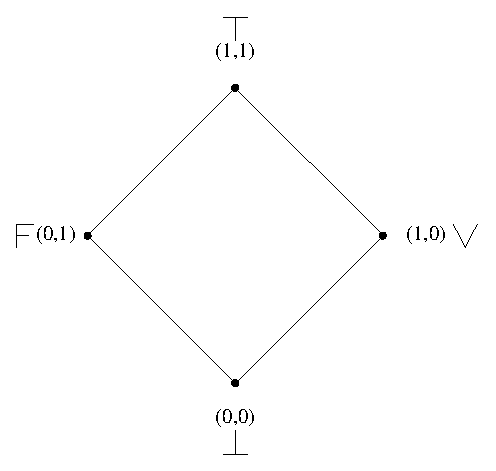
\includegraphics[scale=1.0]{./imagens/C421reticuladoHasse.eps}
%\label{fig:reticuladoHasse1}
%{\small Fonte: \cite{JoaoInacio} }
%\end{figure}


\begin{figure}[!h]
\centering
\caption{Representação do reticulado finito de Hasse }
\begin{tikzpicture}[scale=0.6]
\tikzset{ >=latex, inner sep=0pt, outer sep=0pt,  }

%\draw [lightgray, dashed](0,0) grid (10,10);

\node at (5.0,9.5) {$(1,1)$};
\node at (9.9,4.8) {$(1,0)$};
\node at (5.0,0.5) {$(0,0)$};
\node at (0.1,4.8) {$(0,1)$};

\node at (5.0,10.2) {$\top$};
\node at (9.9,5.5) {V};
\node at (5.0,-0.2) {$\bot$};
\node at (0.1,5.5) {F};

\node [fill=black, circle] (V) at (9,5) {:};
\node [fill=black, circle] (F) at (1,5) {:};
\node [fill=black, circle] (T) at (5,9) {:};
\node [fill=black, circle] (L) at (5,1) {:};

\draw [thick] (V) -- (T);
\draw [thick] (T) -- (F);
\draw [thick] (F) -- (L);
\draw [thick] (L) -- (V);

\end{tikzpicture}
\label{fig:reticuladoHasse}

{\small Fonte: \cite{JoaoInacio}}
\end{figure}








Para toda proposição $P$ há um par de valores, chamada de anotação, $(\mu , \lambda )$, onde $\mu$ é o grau de evidência favorável e $\lambda $ é o grau de evidência contrária, representada como  $P_{( \mu , \lambda )}$ \cite{Abe2014} .

%$P_{( \mu , \lambda )}$
Como exemplificação, para uma proposição $P \equiv$ \emph{"A velocidade de rotação do motor atingiu o valor desejado."}, assume-se dois especialistas para realizarem a leitura dos valores da anotação. Em um sistema físico, os especialistas geralmente são sensores, como neste caso, poderia ser um encoder ou sensor óptico como contador de voltas associado a uma base de tempo.

\begin{itemize}
\item 
$\mu$ = grau de evidência favorável (especialista 1), ou seja, com quanto de certeza, em um intervalo fechado $[0,1]$, sendo 0 para grau nulo de certeza e 1 grau máximo de certeza para a dada proposição $P$;

\item
$\lambda$ = grau de evidência contrária (especialista 2), ou seja, com quanto de certeza, em um intervalo fechado $[0,1]$, sendo 0 o grau nulo de certeza à evidência contrária e 1 o grau máximo de certeza à evidência contrária para a dada proposição $P$.

\end{itemize}


Assim, podemos interpretar da seguinte forma os valores da anotação para as posições extremas do reticulado finito de Hasse:

\begin{itemize}
\item 
$(\mu, \lambda ) = (1,0)$ : Há um grau de evidência favorável total e um grau de evidencia contrária nulo, ou seja, a afirmação da proposição é máxima e sua negação é nula, assim,  $P$ é \emph{Verdadeira} e \emph{A velocidade de rotação do motor atingiu o valor desejado};

\item 
$(\mu, \lambda ) = (0,1)$ : Há um grau de evidência favorável nulo e um grau de evidencia contrária máximo, ou seja, a afirmação da proposição é nula e sua negação é máxima, assim,  $P$ é \emph{Falsa} e \emph{A velocidade de rotação do motor não atingiu o valor desejado};

\item 
$(\mu, \lambda ) = (1,1)$ : Há um grau de evidência favorável máximo e também um grau de evidencia contrária máximo, ou seja, a afirmação da proposição é máxima e sua negação também é máxima, assim,  $P$ é \emph{Inconsistente} e \emph{A velocidade de rotação do motor atingiu e não atigiu o valor desejado}, contradição;

\item 
$(\mu, \lambda ) = (0,0)$ : Há um grau de evidência favorável nulo e também um grau de evidencia contrária nulo, ou seja, a afirmação da proposição é nula e sua negação também é nula, assim,  $P$ é \emph{Indeterminada} e \emph{A velocidade de rotação do motor nem atingiu o valor desejado e nem não atingiu o valor desejado}, situação paracompleta.

\end{itemize}

Os graus de evidência podem assumir valores não extremos:

\begin{itemize}
\item 
$(\mu, \lambda ) = (0.8,0.3)$ : Crê-se com grau de evidência favorável de 80\% e um grau de evidencia contrária de 30\%  que \emph{A velocidade rotação do motor atingiu do valor desejado}.
\end{itemize}

\subsubsection{Operações Lógicas}

Algumas operações lógicas booleanas são definidas 
a partir de duas anotações 
$(\mu _1, \lambda _1)$ e $(\mu _2, \lambda _2)$ 
pertencentes a mesma proposição P 
\cite{JISFeAS} \cite{Abe2014},
aqui denominadas respectivamente $P_1$ e $P_2$:

\begin{itemize}

\item Negação: $\sim$$P _1$ = $(\lambda _1, \mu _1)$ ou 
$\neg$$P _1$ = $(\lambda _1, \mu _1)$

\item Disjunção: $P _1 \vee P _2 = 
(min\{\mu _1, \mu _2\},max\{\lambda _1, \lambda _2\})$ 

\item Conjunção: $P _1 \wedge P _2 = 
(max\{\mu _1, \mu _2\},min\{\lambda _1, \lambda _2\})$ 


\end{itemize}




%%%%%%%%%%%%%%%%%%%%%%%%%%%%%%%%%%%%%%%%%%%%%%%%%%%%%%%%%%%%
\subsection{Quadrado Unitário no Plano Cartesiano - QUPC}
%%%%%%%%%%%%%%%%%%%%%%%%%%%%%%%%%%%%%%%%%%%%%%%%%%%%%%%%%%%%
\nomenclature{$QUPC$}{Quadrado Unitário no Plano Cartesiano}

Uma outra forma de representação da anotação é utilizando o Quadrado Unitário no Plano Cartesiano (QUPC) no qual são transpostos os pontos extremos às respectivas posições de acordo com o par ordenado,  $(\mu, \lambda ) \leftrightarrow (x,y) $, assim o eixo $x$ corresponde ao grau de evidência favorável e o eixo $y$ corresponde ao grau de evidência contrária, conforme mostrado na Figura \ref{fig:reticuladoQUPC}.






\begin{figure}[!h]
\centering
\caption{Representação do reticulado no quadrado unitário no plano cartesiano}
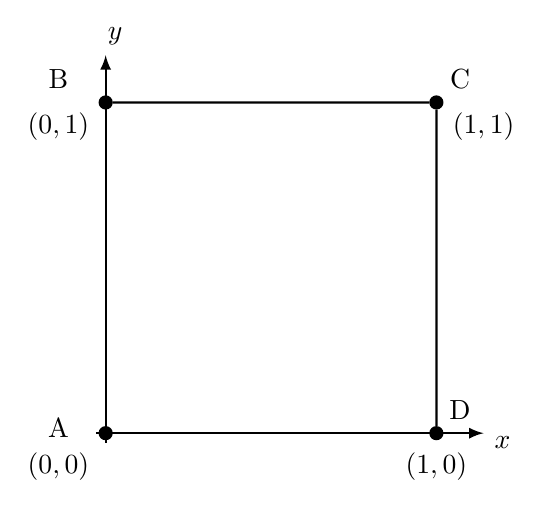
\begin{tikzpicture}[scale=0.6]
\tikzset{ >=latex, inner sep=0pt, outer sep=0pt,  }

%\draw [lightgray, dashed](0,0) grid (10,10);

\node at (1.2,9.4) {$y$};
\node at (9.4,0.8) {$x$};

\node at (0.0,0.3) {$(0,0)$};%A
\node at (0.0,7.5) {$(0,1)$};%B
\node at (9.0,7.5) {$(1,1)$};%C
\node at (8.0,0.3) {$(1,0)$};%D

\node at (0.0,1.1) {A};
\node at (0.0,8.5) {B};
\node at (8.5,8.5) {C};
\node at (8.5,1.5) {D};

\node [fill=black, circle] (V) at (8,1) {:};
\node [fill=black, circle] (F) at (1,8) {:};
\node [fill=black, circle] (T) at (8,8) {:};
\node [fill=black, circle] (L) at (1,1) {:};

\draw [thick] (V) -- (T);
\draw [thick] (T) -- (F);
\draw [thick] (F) -- (L);
\draw [thick] (L) -- (V);

\draw [->, thick] (0.8,1.0) -- (9.0,1.0);
\draw [->, thick] (1.0,0.8) -- (1.0,9.0);

\end{tikzpicture}
\label{fig:reticuladoQUPC}

{\small Fonte: \cite{JoaoInacio} }
\end{figure}







Os pontos extremos assim representam:

\begin{itemize}
\item $A: (0,0) = \bot \Rightarrow $ Paracompleto;
\item $B: (0,1) = F \Rightarrow $ Falso;
\item $C: (1,1) = \top \Rightarrow $ Inconsistente;
\item $D: (1,0) = V \Rightarrow $ Verdade.
\end{itemize}

O segmento de reta $\overline{BD}$, entre os pontos referentes às condições $Verdade$ e $Falso$, conforme mostrado na Figura \ref{fig:retaPerfeitamenteDefinida}, é denominada de \emph{Reta Perfeitamente Definida} e dada uma anotação $(\mu, \lambda )$ situada nela, a soma das evidências anotadas é sempre o valor unitário do quadro. 

%\begin{figure}[!htb]
%\caption{Representação da Reta Perfeitamente Definida}
%\center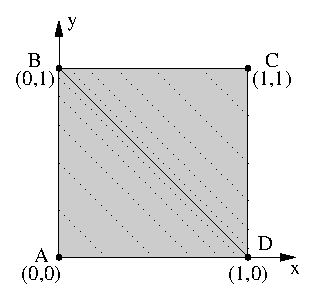
\includegraphics[scale=1.25]{./imagens/C424retaPerfeitamenteDefinida.eps}
%\label{fig:retaPerfeitamenteDefinida1}
%
%{\small Fonte: \cite{JoaoInacio}}
%\end{figure}

\begin{figure}[!h]
\centering
\caption{Representação da Reta Perfeitamente Definida}
\begin{tikzpicture}[scale=0.6]
\tikzset{ >=latex, inner sep=0pt, outer sep=0pt,  }

%\draw [lightgray, dashed](0,0) grid (10,10);

\node at (1.2,9.4) {$\lambda$};
\node at (9.4,0.8) {$\mu$};

\node at (0.0,0.3) {$(0,0)$};%A
\node at (0.0,7.5) {$(0,1)$};%B
\node at (9.0,7.5) {$(1,1)$};%C
\node at (8.0,0.3) {$(1,0)$};%D

\node at (0.0,1.1) {A};
\node at (0.0,8.5) {B};
\node at (8.5,8.5) {C};
\node at (8.5,1.5) {D};

\draw [gray,thick] (V) -- (T);
\draw [gray,thick] (T) -- (F);
\draw [gray,thick] (F) -- (L);
\draw [gray,thick] (L) -- (V);
\draw [] (F) -- (V);

\draw [->,gray, thick] (0.8,1.0) -- (9.0,1.0);
\draw [->,gray, thick] (1.0,0.8) -- (1.0,9.0);

\node [fill=black, circle] (V) at (8,1) {:};
\node [fill=black, circle] (F) at (1,8) {:};
\node [fill=black, circle] (T) at (8,8) {:};
\node [fill=black, circle] (L) at (1,1) {:};

\end{tikzpicture}
\label{fig:retaPerfeitamenteDefinida}

{\small Fonte: \cite{JoaoInacio}}
\end{figure}








A relação dos graus de evidência da anotação quando coincidente à Reta Perfeitamente Definida é: 

\begin{center}
\begin{equation}
\mu + \lambda = 1
\label{eq:evidenciaUnitaria1}
\end{equation}
\end{center}

Assim, temos que:

\begin{center}
\begin{equation}
\mu + \lambda - 1 = 0
\label{eq:evidenciaUnitaria}
\end{equation}
\end{center}


Os graus de evidência não precisam apresentar valores complementares, possuem independência entre si, assim das Equações  
\ref{eq:evidenciaUnitaria1} e 
\ref{eq:evidenciaUnitaria} 
é elaborado o conceito de 
\emph{Grau de Incerteza}($G_{in}$), 
e temos que: 

\nomenclature{$G_{in}$}{Grau de Incerteza}

\begin{center}
\begin{equation}
G_{in} = \mu + \lambda - 1
\label{eq:grauContradicao}
\end{equation}
\end{center}

pois quanto mais próximo da Reta Perfeitamente Definida, menor é o grau de incerteza apresentado pelos graus de evidência, sendo zero quando não houver inconsistência e o ponto de anotação situar-se sobre a Reta Perfeitamente Definida. 
Quanto mais afastado da Reta Perfeitamente Definida estiver o ponto de anotação, e mais próximo aos pontos A ou C, maior é o Grau de Incerteza. 

Quando a anotação estiver situada na região entre os pontos BCD, acima da reta perfeitamente definida, o Grau de Incerteza é denominado 
\emph{Grau de Inconsistência} ($G_{ic}$), 
e isso ocorre quando, $\mu \ge \lambda $, de forma oposta, quando $\mu < \lambda $ a anotação está situada na região entre os pontos BAD, abaixo da reta perfeitamente definida, e o grau de Incerteza é denominado 
\emph{Grau de Paracompleteza} ($G_{pa}$), 
então pode-se dizer que:

\nomenclature{$G_{pa}$}{Grau de Paracompleteza}
\nomenclature{$G_{ic}$}{Grau de Inconsistência}

\begin{center}
\begin{equation}
-1 \le G _{pa}  <  0 \le G _{ic} \le 1
\label{eq:grauInconsistenciaIndefinicao}
\end{equation}
\end{center}
e
\begin{center}
\begin{equation}
-1 \le G _{in} \le 1
\label{eq:grauInconsistenciaIndefinicao1}
\end{equation}
\end{center}


O segmento de reta $\overline{ AC }$ , entre os pontos referentes às
condições \emph{Paracompletude} e \emph{Inconsistência}, conforme mostrado
na Figura \ref{fig:retaPerfeitamenteIndefinida}, é denominada de
\emph{Reta Perfeitamente Indefinida} e dada uma anotação $(\mu,
\lambda )$ situada nela, a subtração das evidências anotadas é sempre
zero, ou seja, $\mu = \lambda$, e de forma contrária,
quando a anotação está posicionada de forma não coincidente à Reta
Perfeitamente Indefinida,
significa que $\mu \neq \lambda$.

%\begin{figure}[!htb]
%\caption{Representação da Reta Perfeitamente Indefinida}
%\center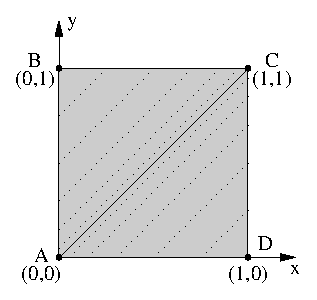
\includegraphics[scale=1.25]{./imagens/C426retaPerfeitamenteIndefinida.eps}
%\label{fig:retaPerfeitamenteIndefinida1}
%
%{\small Fonte: \cite{JoaoInacio} }
%\end{figure}



\begin{figure}[!h]
\centering
\caption{Representação da Reta Perfeitamente Indefinida}
\begin{tikzpicture}[scale=0.6]
\tikzset{ >=latex, inner sep=0pt, outer sep=0pt,  }

%\draw [lightgray, dashed](0,0) grid (10,10);

\node at (1.2,9.4) {$\lambda$};
\node at (9.4,0.8) {$\mu$};

\node at (0.0,0.3) {$(0,0)$};%A
\node at (0.0,7.5) {$(0,1)$};%B
\node at (9.0,7.5) {$(1,1)$};%C
\node at (8.0,0.3) {$(1,0)$};%D

\node at (0.0,1.1) {A};
\node at (0.0,8.5) {B};
\node at (8.5,8.5) {C};
\node at (8.5,1.5) {D};

\draw [gray,thick] (V) -- (T);
\draw [gray,thick] (T) -- (F);
\draw [gray,thick] (F) -- (L);
\draw [gray,thick] (L) -- (V);
\draw [thick] (T) -- (L);

\draw [->,gray, thick] (0.8,1.0) -- (9.0,1.0);
\draw [->,gray, thick] (1.0,0.8) -- (1.0,9.0);

\node [fill=black, circle] (V) at (8,1) {:};
\node [fill=black, circle] (F) at (1,8) {:};
\node [fill=black, circle] (T) at (8,8) {:};
\node [fill=black, circle] (L) at (1,1) {:};

\end{tikzpicture}
\label{fig:retaPerfeitamenteIndefinida}

{\small Fonte: \cite{JoaoInacio} }
\end{figure}











A relação dos graus de evidência para uma anotação cuja posição coincide com a Reta Perfeitamente Indefinida é: 

\begin{center}
\begin{equation}
\mu - \lambda = 0
\label{eq:evidenciaIndefinida}
\end{equation}
\end{center}

De forma análoga ao Grau de Inconsistência, da Equação \ref{eq:evidenciaIndefinida} é elaborado o conceito de \emph{Grau de Certeza} ($G_{ce}$), assim temos que: 

\nomenclature{$G_{ce}$}{Grau de Certeza}

\begin{center}
\begin{equation}
G _{ce} = \mu - \lambda
\label{eq:grauCerteza}
\end{equation}
\end{center}

Quando os graus de evidência, favorável e contrário, são iguais, não há certeza em relação à proposição, mas quando são diferentes, alguma certeza pode ser inferida, até a condição máxima onde uma das evidências é total (1) e a outra é nula (0), caracterizando a condição verdadeira ou falsa, afastando o ponto anotado da Reta Perfeitamente Indefinida. 

Quando a anotação situa-se entre os pontos ABC do QUPC, o grau de certeza é denominado \emph{Grau de Falsidade ($G _{fa}$)}, e tal condição ocorre quando $\mu < \lambda $, caso contrário, se $\mu \ge \lambda $, a anotação situa-se entre os pontos ACD do QUPC, e o grau de certeza é denominado \emph{Grau de Veracidade ($G _{ve})$}, então pode-se dizer que:

\nomenclature{$G_{fa}$}{Grau de Falsidade}
\nomenclature{$G_{ve}$}{Grau de Veracidade}

\begin{center}
\begin{equation}
-1 \le G_{fa}  <  0 \le G_{ve} \le 1
\label{eq:grauVerdadeFalsidade}
\end{equation}
\end{center}
e
\begin{center}
\begin{equation}
-1 \le G_{ce} \le 1
\label{eq:grauCertezaIntervalo}
\end{equation}
\end{center}

Graficamente são representadas como mostra a Figura \ref{fig:retasgcgct}:

%\begin{figure}[!htb]
%\caption{Representação dos Graus de Certeza e Incerteza em um plano cartesiano}
%\center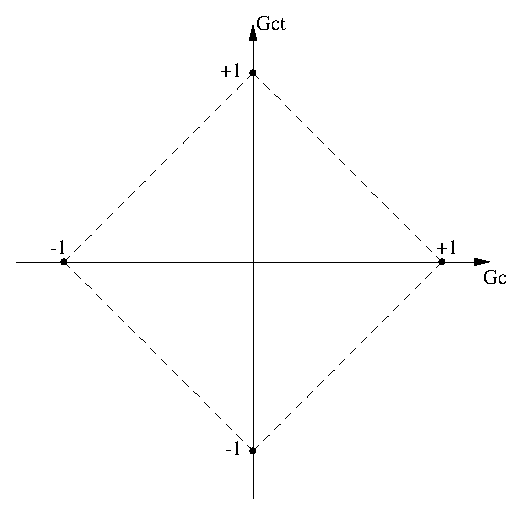
\includegraphics[scale=1.0]{./imagens/C428retasgcgct.eps}
%\label{fig:retasgcgct1}
%
%{\small Fonte: \cite{JoaoInacio}}
%\end{figure}

\begin{figure}[!h]
\centering
\caption{Representação dos Graus de Certeza e Incerteza em um plano cartesiano}
\begin{tikzpicture}[scale=0.8]
\tikzset{ >=latex, inner sep=0pt, outer sep=0pt,  }

%\draw [lightgray, dashed](0,0) grid (10,10);

\node at ( 5.5,10.0) {$G_{in}$};
\node at (10.0, 5.5) {$G_{ce}$};

\node at (9.0,4.5) {$+1$};
\node at (0.5,5.5) {$-1$};
\node at (4.5,9.4) {$+1$};
\node at (4.5,0.6) {$-1$};

\draw [->,gray, thick] (5.0,0.0) -- ( 5.0,10.0);
\draw [->,gray, thick] (0.0,5.0) -- (10.0, 5.0);

\node [fill=black, circle] (V) at (9,5) {.};
\node [fill=black, circle] (F) at (1,5) {.};
\node [fill=black, circle] (T) at (5,9) {.};
\node [fill=black, circle] (L) at (5,1) {.};

\draw [dashed] (V)--(T);
\draw [dashed] (T)--(F);
\draw [dashed] (F)--(L);
\draw [dashed] (L)--(V);

\end{tikzpicture}
\label{fig:retasgcgct}

{\small Fonte: \cite{JoaoInacio}}
\end{figure}











A representação ainda é dividia em algumas partes, dependendo da aplicação, estabelecendo quais são os limites que definem cada estado, Verdadeiro, Falso, Paracompleto, Inconsistente e outros mais que forem pertinentes à aplicação, estão representados pelas linhas tracejadas na Figura \ref{fig:valorControle} e são definidos como:

\begin{itemize}
\item \emph{$V_{scc}$ : Valor limite superior de Controle de Certeza};
\item \emph{$V_{icc}$ : Valor limite inferior de Controle de Certeza};
\item \emph{$V_{sci}$ : Valor limite superior de Controle de Incerteza};
\item \emph{$V_{ici}$ : Valor limite inferior de Controle de Incerteza}.
\end{itemize}

\nomenclature{$V_{scc}$}{ Valor limite superior de controle de certeza}
\nomenclature{$V_{icc}$}{ Valor limite inferior de controle de certeza}
\nomenclature{$V_{sci}$}{ Valor limite superior de controle de incerteza}
\nomenclature{$V_{ici}$}{ Valor limite inferior de controle de incerteza}


%\begin{figure}[!htb]
%\caption{Representação dos valores de controle}
%\center\includegraphics[scale=1.0]{./imagens/C429valorControle.eps}
%\label{fig:valorControle1}
%
%{\small Fonte: \cite{JoaoInacio}}
%\end{figure}

\begin{figure}[!h]
\centering
\caption{Representação dos valores de controle}
\begin{tikzpicture}[scale=0.8]
\tikzset{ >=latex, inner sep=0pt, outer sep=0pt,  }

%\draw [lightgray, dashed](0,0) grid (10,10);

\node at ( 5.5,10.0) {$G_{in}$};
\node at (10.0, 5.5) {$G_{ce}$};

\node at (9.0,4.5) {$+1$};
\node at (0.5,5.5) {$-1$};
\node at (4.5,9.4) {$+1$};
\node at (4.5,0.6) {$-1$};

\draw [->, thick] (5.0,0.0) -- ( 5.0,10.0);
\draw [->, thick] (0.0,5.0) -- (10.0, 5.0);

\node [fill=black, circle] (V) at (9,5) {.};
\node [fill=black, circle] (F) at (1,5) {.};
\node [fill=black, circle] (T) at (5,9) {.};
\node [fill=black, circle] (L) at (5,1) {.};

\draw [thick] (V)--(T);
\draw [thick] (T)--(F);
\draw [thick] (F)--(L);
\draw [thick] (L)--(V);

\draw [dashed] (7,7)--(3,7)--(3,3)--(7,3)--(7,7);

\end{tikzpicture}
\label{fig:valorControle}

{\small Fonte: \cite{JoaoInacio}}
\end{figure}














Uma divisão em 12 partes é mostrada na Figura \ref{fig:reticuladoLPA2v} com seus respectivos estados intermediários definidos conforme \citeauthor{JoaoInacio}(\citeyear{JoaoInacio}), sendo 4 regiões extremas:


%\begin{figure}[!htb]
%\center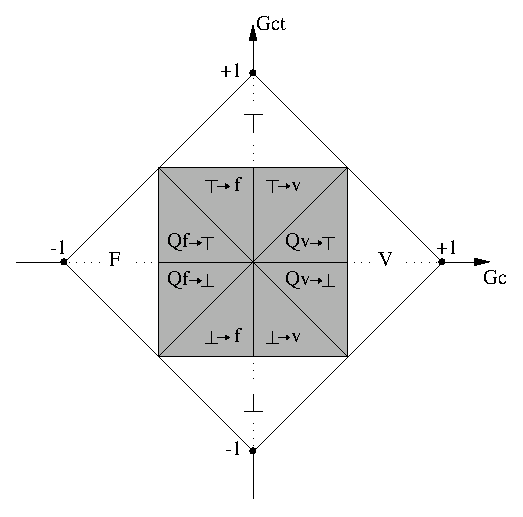
\includegraphics[scale=1.5]{./pic/C430gcgct.eps}
%\caption{Representação do reticulado da LPA2v subdividido em 12 regiões}
%\label{fig:reticuladoLPA2v}
%\end{figure}


\begin{figure}[!h]
\centering
\caption{Representação do reticulado da Lógica $E\tau$ subdividido em 12 regiões}
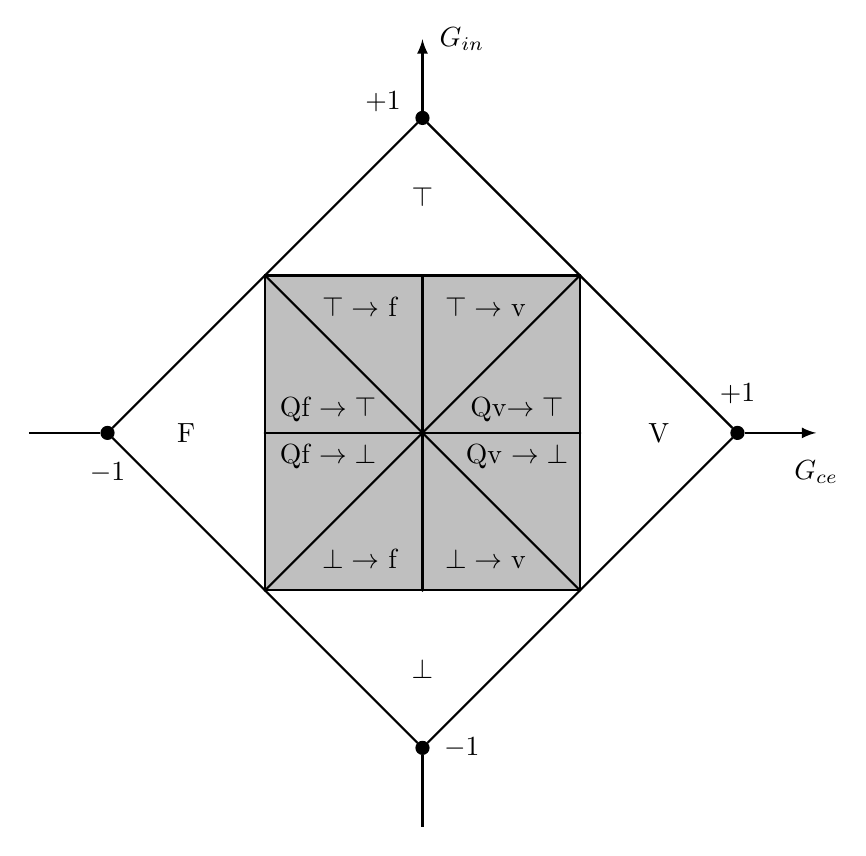
\begin{tikzpicture}[scale=1.0]
\tikzset{ >=latex, inner sep=0pt, outer sep=0pt,  }

%\draw [lightgray, dashed](0,0) grid (10,10);

\node [fill=black, circle] (V) at (9,5) {:};
\node [fill=black, circle] (F) at (1,5) {:};
\node [fill=black, circle] (T) at (5,9) {:};
\node [fill=black, circle] (L) at (5,1) {:};

\node [fill=black, circle] (N) at (5,7) { };
\node [fill=black, circle] (S) at (5,3) { };
\node [fill=black, circle] (E) at (7,5) { };
\node [fill=black, circle] (W) at (3,5) { };

\node [fill=black, circle] (NE) at (7,7) { };
\node [fill=black, circle] (SE) at (7,3) { };
\node [fill=black, circle] (NW) at (3,7) { };
\node [fill=black, circle] (SW) at (3,3) { };


%\draw [dashed] (F) -- (V);
%\draw [dashed] (T) -- (L);
\draw [->, thick] (V)   -- (10,5);
\draw [    thick] (0,5) -- (F);
\draw [->, thick] (T)   -- (5,10);
\draw [    thick] (5,0) -- (L);

\draw [thick] (V) -- (T);
\draw [thick] (T) -- (F);
\draw [thick] (F) -- (L);
\draw [thick] (L) -- (V);

\draw [thick] (N) -- (S);
\draw [thick] (E) -- (W);
\draw [thick] (NE) -- (SW);
\draw [thick] (SE) -- (NW);


\draw[thick] (SW) rectangle (NE);
\fill[nearly transparent] (SW) rectangle (NE);

\node at (8,5) {V};
\node at (2,5) {F};
\node at (5,8) {$\top$};
\node at (5,2) {$\bot$};

\node at (6.2,5.3) {Qv$\rightarrow\top$ };
\node at (6.2,4.7) {Qv $\rightarrow  \bot$ };
\node at (3.8,5.3) {Qf $\rightarrow  \top$ };
\node at (3.8,4.7) {Qf $\rightarrow  \bot$ };
\node at (4.2,6.6) {$\top \rightarrow $ f };
\node at (5.8,6.6) {$\top \rightarrow $ v };
\node at (4.2,3.4) {$\bot \rightarrow $ f };
\node at (5.8,3.4) {$\bot \rightarrow $ v };

\node at (10,4.5) {$G_{ce}$};
\node at (5.5,10) {$G_{in}$};

\node at (4.5,9.2) {$+1$};
\node at (9.0,5.5) {$+1$};
\node at (5.5,1.0) {$-1$};
\node at (1.0,4.5) {$-1$};

\end{tikzpicture}
\label{fig:reticuladoLPA2v}

{\small Fonte: \cite{JoaoInacio} }
\end{figure}




\begin{itemize}
\item V : Verdadeiro;
\item F : Falso;
\item $\top$ : Inconsistente;
\item $\bot$ : Paracompleto.
\end{itemize}
e 8 regiões intermediárias: 
\begin{itemize}
\item Qv $\rightarrow  \top$ : Quase Verdade tendendo à Inconsistência;
\item Qv $\rightarrow  \bot$ : Quase Verdade tendendo à  Paracompletude;
\item Qf $\rightarrow  \top$ : Quase Falso tendendo à Inconsistência;
\item Qf $\rightarrow  \bot$ : Quase Falso tendendo à Paracompletude;
\item $\top \rightarrow $ f : Inconsistência tendendo à Falsidade;
\item $\top \rightarrow $ v : Inconsistência tendendo à Veracidade;
\item $\bot \rightarrow $ f : Paracompleto tendendo à Falsidade;
\item $\bot \rightarrow $ v : Paracompleto tendendo à Veracidade.

\end{itemize}

O reticulado subdividido em 12 regiões como mostrado, é aplicado em situações nas quais a tomada de decisão utiliza estados discretos bem definidos para atuação, onde para cada posição da anotação e respectivamente um estado do reticulado, uma ação é tomada, assim sendo, a quantidade de subdivisões está fortemente dependente da aplicação.


O reticulado pode ser dividido de outras formas, dependendo dos limites dos Graus de Certeza e Incerteza que o sistema permite. A Figura \ref{fig:reticuladoLPA2v2} mostra uma das possibilidades com a representação de 8 regiões do reticulado. 


\begin{figure}[!h]
\centering
\caption{Representação do reticulado da Lógica $E\tau$ subdividido em 8 regiões}
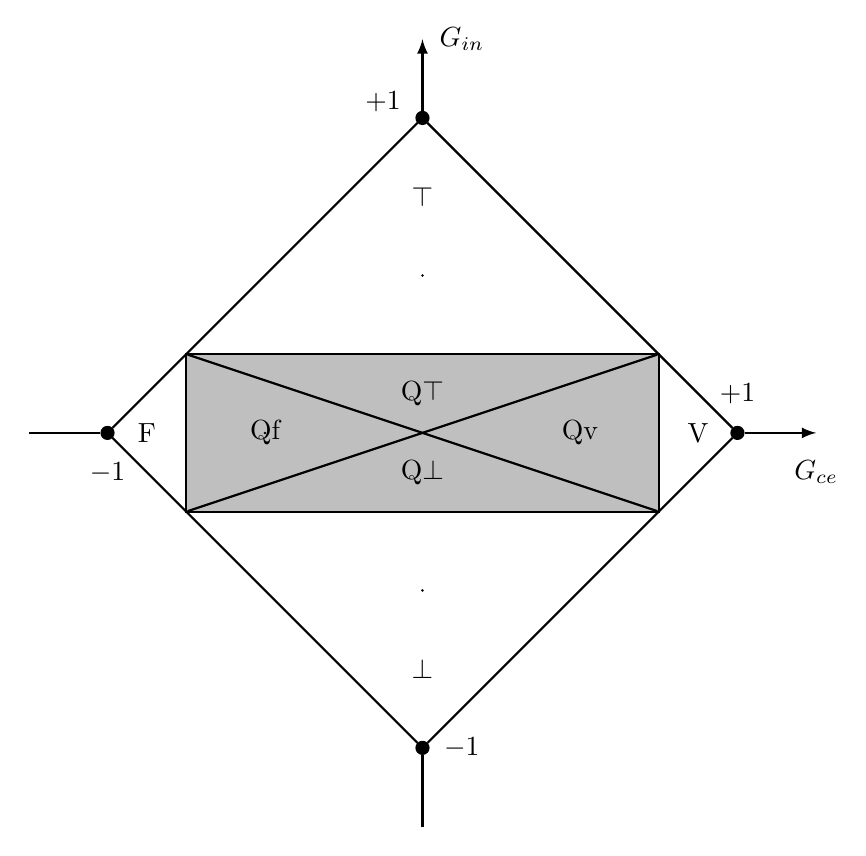
\begin{tikzpicture}[scale=1.0]
\tikzset{ >=latex, inner sep=0pt, outer sep=0pt,  }

%\draw [lightgray, dashed](0,0) grid (10,10);

\node at (10,4.5) {$G_{ce}$};
\node at (5.5,10) {$G_{in}$};

\node at (4.5,9.2) {$+1$};
\node at (9.0,5.5) {$+1$};
\node at (5.5,1.0) {$-1$};
\node at (1.0,4.5) {$-1$};

\node [fill=black, circle] (V) at (9,5) {:};
\node [fill=black, circle] (F) at (1,5) {:};
\node [fill=black, circle] (T) at (5,9) {:};
\node [fill=black, circle] (L) at (5,1) {:};

\node [fill=black, circle] (N) at (5,7) { };
\node [fill=black, circle] (S) at (5,3) { };
\node [fill=black, circle] (E) at (7,5) { };
\node [fill=black, circle] (W) at (3,5) { };

\node [fill=black, circle] (NE) at (8,6) { };
\node [fill=black, circle] (SE) at (8,4) { };
\node [fill=black, circle] (NW) at (2,6) { };
\node [fill=black, circle] (SW) at (2,4) { };

\draw [->, thick] (V)   -- (10,5);
\draw [    thick] (0,5) -- (F);
\draw [->, thick] (T)   -- (5,10);
\draw [    thick] (5,0) -- (L);

\draw [thick] (V) -- (T);
\draw [thick] (T) -- (F);
\draw [thick] (F) -- (L);
\draw [thick] (L) -- (V);

\draw [thick] (NE) -- (SW);
\draw [thick] (SE) -- (NW);

\draw[thick] (SW) rectangle (NE);
\fill[nearly transparent] (SW) rectangle (NE);

\node at (8.5,5.0) {V};
\node at (1.5,5.0) {F};
\node at (5.0,8.0) {$\top$};
\node at (5.0,2.0) {$\bot$};

\node at (7.0,5.0) {Qv};
\node at (3.0,5.0) {Qf};
\node at (5.0,5.5) {Q$\top$};
\node at (5.0,4.5) {Q$\bot$};

\end{tikzpicture}
\label{fig:reticuladoLPA2v2}

{\small Fonte: Próprio autor}
\end{figure}

Sendo 4 regiões extremas,
\begin{itemize}
\item V : Verdadeiro;
\item F : Falso;
\item $\top$ : Inconsistente;
\item $\bot$ : Paracompleto.
\end{itemize}
e 4 regiões intermediárias: 
\begin{itemize}
\item Qv: Quase Verdade;
\item Qf: Quase Falso;
\item Q$\top$: Quase Inconsistente;
\item Q$\bot$: Quase Paracompleto.

\end{itemize}


%###

É possível e desejável que se possa utilizar um valor resultante que
exclua os efeitos das paracompletudes ou inconsistências \cite{JairJoaoGermano}:

\begin{citacao}
{
"Um sistema de decisão capaz de analisar dados originários de Conhecimento Incerto terá maior robustez quando, 
ao final da análise,
apresentar um resultado que represente o valor de certeza puro, 
isto é, não contaminado pelos efeitos das incertezas."
}
\end{citacao}

O valor que elimina o efeito da incerteza é denominado \emph{Grau de Certeza Real - $G_{CR}$} 
e é calculado pela distância (D) do Ponto de análise, $(G_{ce},G_{in})$, 
em relação ao ponto de máximo Grau de Certeza $V$,
no vértice direito do reticulado, 
conforme mostrado na Figura \ref{fig:reticuladoGer}.

\nomenclature{$G_{CR}$}{Grau de Certeza Real}

\begin{figure}[!h]
\centering
\caption{Representação do Grau de Certeza Real no reticulado }
\begin{tikzpicture}[scale=1.0]
\tikzset{ >=latex, inner sep=0pt, outer sep=0pt,  }

%\draw [lightgray, dashed](0,0) grid (10,10);

\node at (10,4.5) {$G_{ce}$};
\node at (5.5,10) {$G_{in}$};

\node at (4.5,9.2) {$+1$};
\node at (9.0,5.5) {$+1$};
\node at (5.5,1.0) {$-1$};
\node at (1.0,4.5) {$-1$};

\node at (9.0,4.5) {V};
\node at (1.0,5.5) {F};
\node at (5.5,9.0) {$\top$};
\node at (4.5,1.0) {$\bot$};

\node [fill=black, circle] (V) at (9,5) {:};
\node [fill=black, circle] (F) at (1,5) {:};
\node [fill=black, circle] (T) at (5,9) {:};
\node [fill=black, circle] (L) at (5,1) {:};

\draw [thick] (V) -- (T);
\draw [thick] (T) -- (F);
\draw [thick] (F) -- (L);
\draw [thick] (L) -- (V);

\draw [->, thick] (V)   -- (10,5);
\draw [    thick] (0,5) -- (F);
\draw [->, thick] (T)   -- (5,10);
\draw [    thick] (5,0) -- (L);

\draw [lightgray,dashed] (V) -- (F);
\draw [lightgray,dashed] (T) -- (L);

\node [fill=black, circle] (P) at (6.0,7.0) {:};
\node [fill=gray,  circle] (p) at (5.4,5.0) [gray] {:};
\node [fill=black, circle] (r) at (6.0,5.0) [gray]{.};

\draw [blue,ultra thick] (P) -- (V);
\draw [green ] (r) -- (V);
\draw [yellow] (P) -- (r);
%\draw [green,ultra thick] (9.0,4.9) -- (5.4,4.9);

\draw [red, ultra thick,<-]  (p) to [out=85, in=236] (P);

\node at (7.0,6.0) [blue]{D};
\node at (5.7,7.4) {($G_{ce}$,$G_{in}$)};
\node at (5.5,4.6) {$G_{CR}$};

\end{tikzpicture}
\label{fig:reticuladoGer}

{\small Fonte: \cite{JairJoaoGermano}}
\end{figure}


O Grau de Certeza Real ($G_{CR}$) 
é calculado utilizando o Teorema de Pitágoras para achar a distância D 
conforme Equação \ref{eq:grauCertezaReal}. 

\begin{center}
\begin{equation}
D = \sqrt{(1-|G_{ce}|)^2+G_{in}^2}
\label{eq:grauCertezaReal}
\end{equation}
\end{center}

Para valores de $G_{ce} \geq 0$: 

\begin{center}
\begin{equation}
G_{CR} = (1-D)
\end{equation}
\end{center}

Para valores de $G_{ce} < 0$:

\begin{center}
\begin{equation}
G_{CR} = (D-1)
\end{equation}
\end{center}


O Grau de Evidência Real é representado por $\mu_{ER}$ 
e é utilizado para converter o $G_{ce}$ ou $G_{CR}$ 
em uma variável dentro do intervalo fechado $[0,1]$, 
permitindo que o resultado de um bloco LPA$E\tau$ 
possa ser utilizado como entrada em outro bloco. 
Para a conversão é efetuada a equação \ref{eq:muer}:

%\nomenclature{$\mu_{ER}$}{Grau de Evidência Real}

\begin{equation}
\mu_{ER} = \frac{G_{ce} + 1}{2}
\label{eq:muer}
\end{equation}


Tanto o Grau de Certeza Real quanto o Grau de Evidência Real 
ou os estados ou regiões do reticulado 
podem ser utilizados para realizar o controle dos mais diversos tipos de sistemas, 
dependendo apenas do tipo de controle e de sistema que deve ser implementado. 


